\section{Mutation}
In this section, the different types of mutations are described. Mutations introduce new elements in a song, they can have a positive effect, a negative effect or a neutral effect on the total fitness of a song. Some mutations can be seen as optimizations if they guarantee improvement in the total fitness. 

The mutation step is executed if the population become similar. This similarity is calculated by comparing the fitness of the best-rated song with the fitness of the worst-rated song within the population. This value is called the maximum population difference. If this difference is lower than a certain threshold, the population will be mutated, otherwise the mutation step will be skipped. 

Once the population is selected for mutation, a part of the population will be selected for mutation. This is called the "song mutation probability", which is the probability of a song to be selected for mutation.

For each song that is selected for mutation, there is a probability of selecting a particular type of mutation. After executing all the selected mutations on a song, there is a chance for this song to restart the mutation process. This allows the possibility to re-mutate a song multiple times.

\subsection{Neighbour pitch mutation}
This mutation is can be seen as an optimization. Wrong intervals introduced in \ref{sec:rater:neighbourpitch} are being selected for mutation. Out of this selection of intervals, one is randomly chosen for mutation. In order to fix the chosen interval, a note or a chord needs to be transposed. An interval consists of a start note and an end note. For a chord, only the root note is considered for the interval, but the whole chord is transposed if selected. Consider the following notes:
$P$ is previous note before the middle interval, $S$ is the start note of middle interval, $E$ is the end note of middle interval and $N$ is the next note after the middle interval. These four elements create the three following intervals: $PS$ the previous interval, $SE$ the middle interval and the $EN$ next interval. Every interval has a step size called the semitone: the previous semitone, the middle semitone and the next semitone. 
\\
This mutation selects the end note $E$ or the start note $S$ for mutation. There are four cases. The first case is when the absolute value of the next semitone is higher than the previous semitone and the direction of the middle interval is different from the next interval. The direction is the sign of the semitone. This is illustrated at figure \ref{fig:npmut_case1}. Here, the end note $E$ will be transposed upwards.

\begin{figure}[H]
	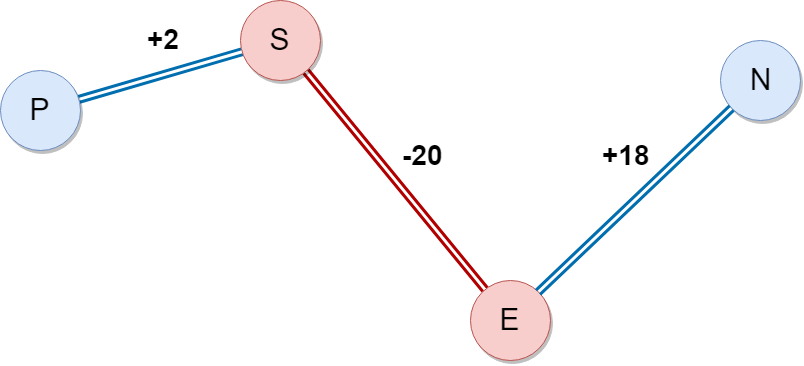
\includegraphics[width=\linewidth]{Fotos/np_mutation/Case1.png}
	\caption{Case where note E is going to be transposed upwards.}
	\label{fig:npmut_case1}
\end{figure}

The next case is illustrated at figure \ref{fig:npmut_case2}. The absolute value of the next semitone is higher than the previous one just like the previous case, but the direction of the middle interval, however, is not different from the next interval. Here, the start note $S$ will be transposed downwards.

\begin{figure}[H]
	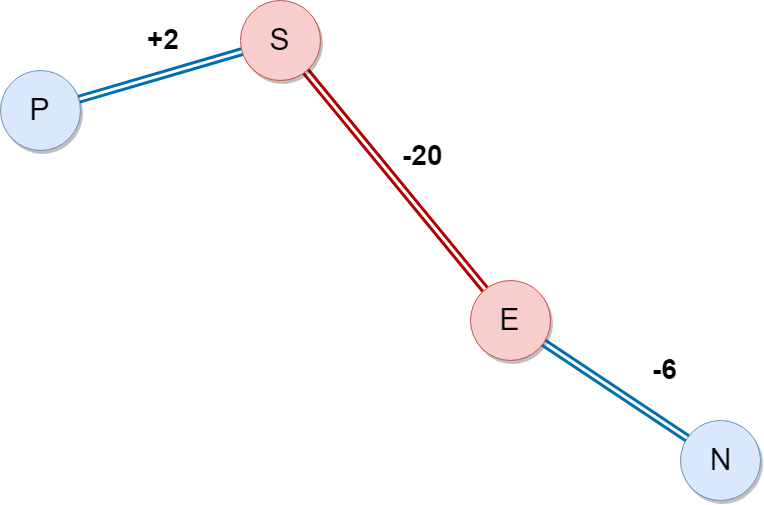
\includegraphics[width=\linewidth]{Fotos/np_mutation/Case2.png}
	\caption{Case where note S is going to be transposed downwards.}
	\label{fig:npmut_case2}
\end{figure}

There are two cases left, they both have similar behavior but in an opposing way. Here, the absolute value of the next semitone is lower than the previous unlike the previous cases. Now the previous interval direction is compared with the middle interval direction. If the direction of the middle interval and previous interval are the same the end note $E$ is selected, else the start note $S$. In all these cases, if the start note is selected, it will be transposed in the direction of the middle interval. If the end note is selected, it will be transposed in the opposite direction of the middle interval. The note will be transposed according to the scale the song tend to follow.
\subsection{Measure swap mutation}
This mutation selects two measures and swaps their place in the song. Consider the measures that are to be swapped measure A and measure B. The selection of measure A will be 50\% of the time random. Half the time the selection of A is random the other half it is somewhat logical.
\\\\
When the selection is random, randomly select a measure in the song for mutation. If the measure selection is not random, the worst measure in the song will be chosen for mutation. The worst measure is based on the scores calculated in section \ref{sec:relmeasurebasedratings}.
\\\\
Measure B is always chosen randomly and measure B must not be equal to measure A. These measures A and B now get swapped in position. The structure of the song will hereby be manipulated.

\subsection{Measure mix mutation}
This mutation selects two measures A an B the same way as the measure swap mutation. After selection, some elements from measure B are copied and placed inside of measure A.


\subsubsection{Element swap mutation}
This mutation is self-evident: two random elements from the song are swapped. Similarly to the measure swap mutation, the purpose of this mutation is to alter the order of elements in the song.

\subsubsection{Element type mutation}
Here, an element (rest, note or chord) from the song is replaced with another already existing element in the song that has a different type. The duration of the note will be unchanged. This mutation has a direct effect on all the scores that are based on the types of the song.

\subsubsection{Element pitch mutation}
This mutation  transposes a note or a chord within the limits. These limits are determined by the master song. This limit is the same as the limit that defines a wrong interval (see section \ref{sec:rater:neighbourpitch}). This has a direct effect on the neighbor pitch rating.


